\documentclass{standalone}
\usepackage{tikz}
\usetikzlibrary{patterns}
\usetikzlibrary{positioning}
\usetikzlibrary{patterns, positioning}
\usetikzlibrary{shapes.misc}
\usepackage[outline]{contour}
\contourlength{1.5pt} 
\usepackage[sfdefault]{ClearSans}

\begin{document}
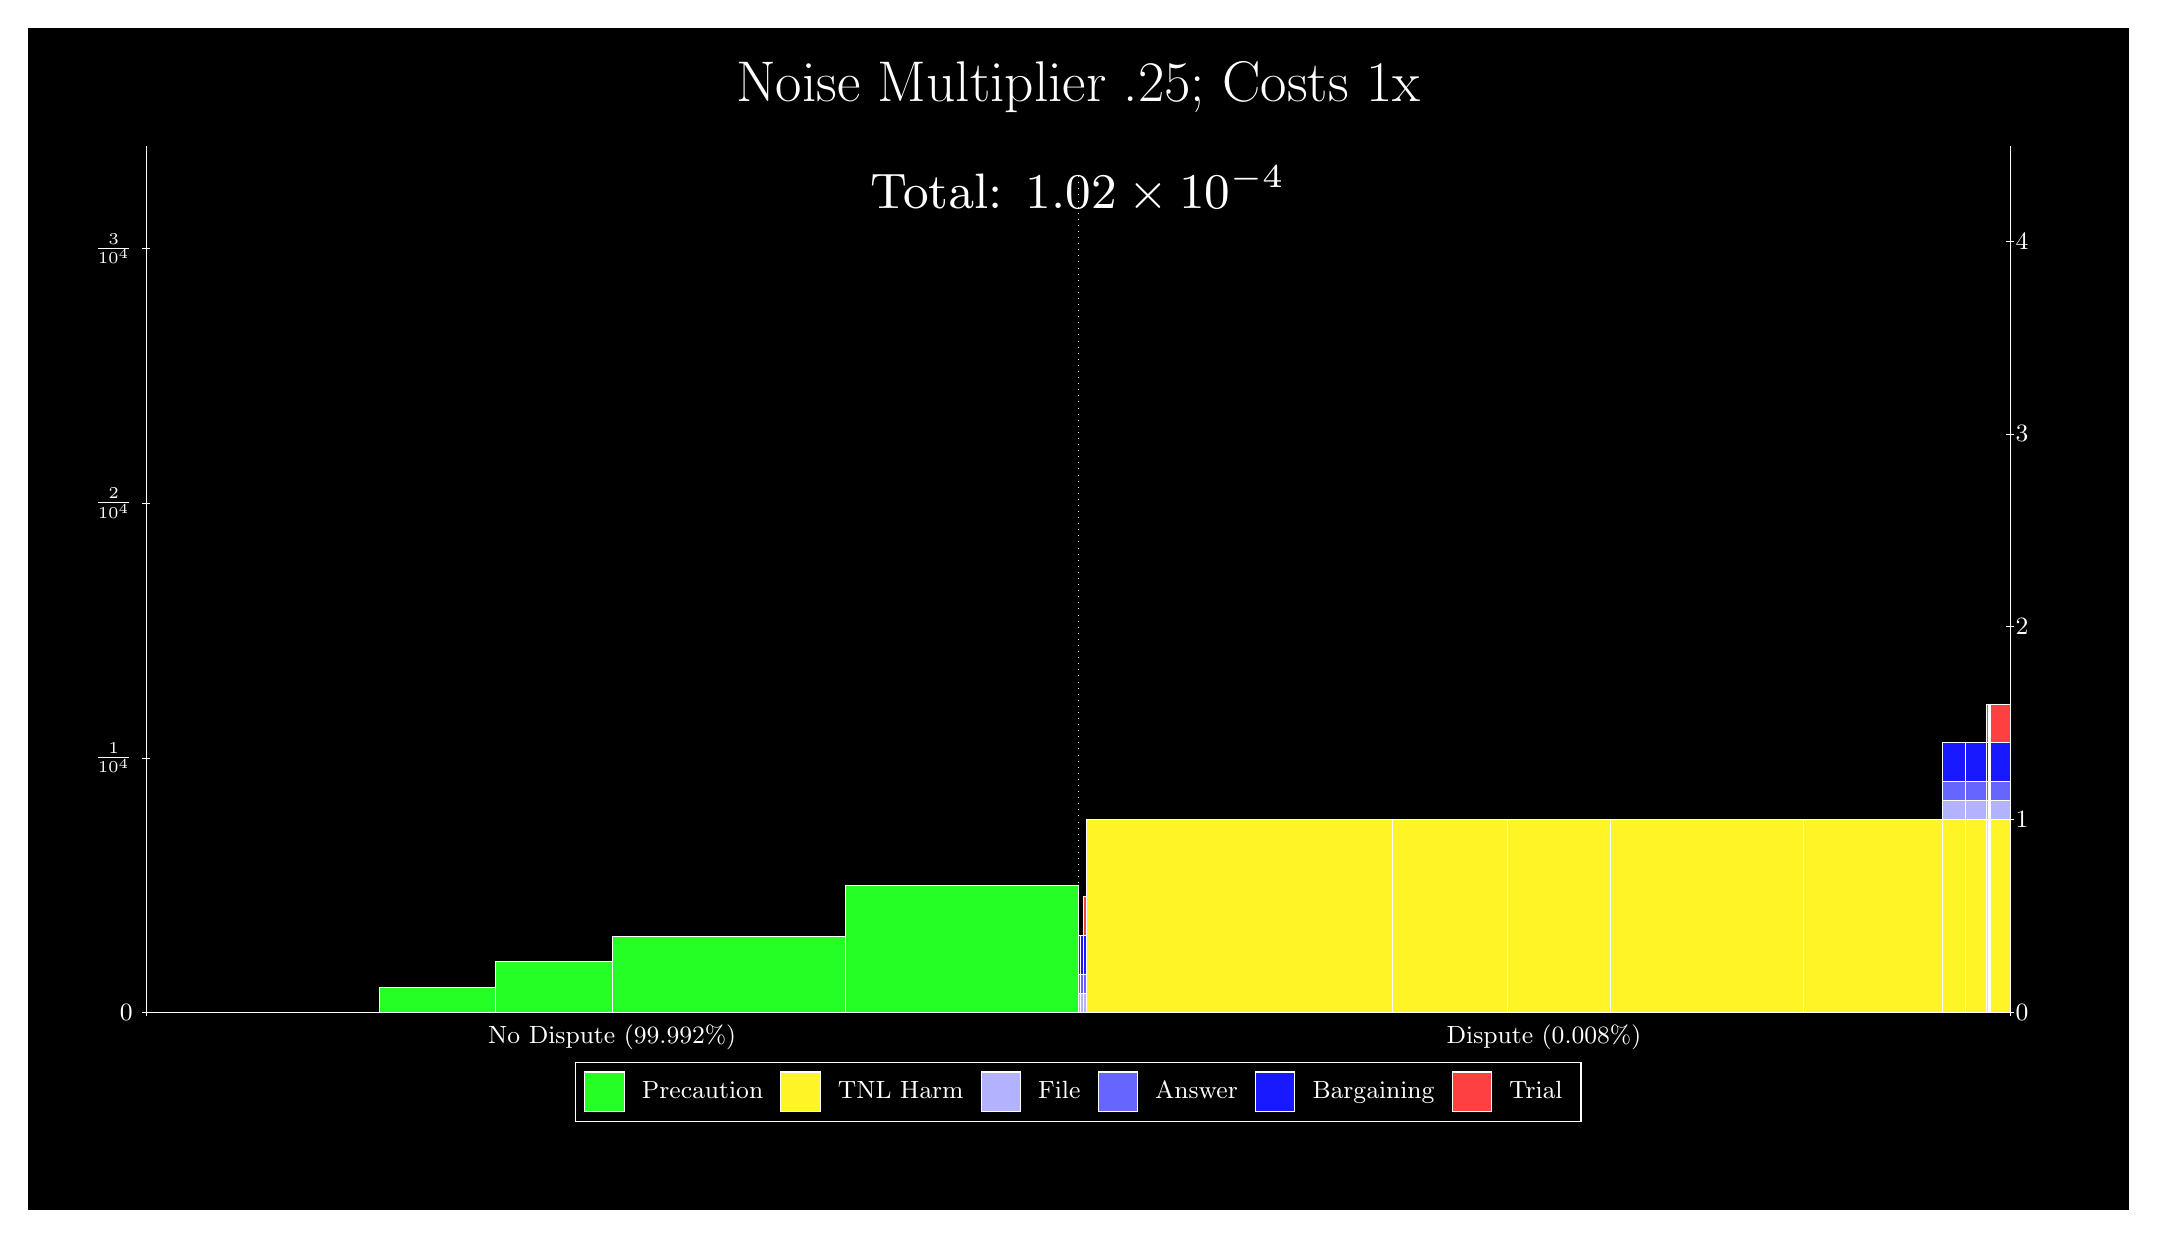
\begin{tikzpicture}
\draw[fill=black] (0,0) rectangle (26.667,15);
\draw[draw=none,text=white] (0,13.5) rectangle (26.667,15) node[midway] {\huge Noise Multiplier .25; Costs 1x};
\draw[fill=green!85,draw=white,very thin] (4.4582,2.5) rectangle (5.9374,2.8234);
\draw[fill=green!85,draw=white,very thin] (5.9374,2.5) rectangle (7.4165,3.1468);
\draw[fill=green!85,draw=white,very thin] (7.4165,2.5) rectangle (10.375,3.4702);
\draw[fill=green!85,draw=white,very thin] (10.375,2.5) rectangle (13.333,4.117);
\draw[fill=green!85,draw=white,very thin] (13.333,2.5) rectangle (13.366,2.5);
\draw[fill=blue!30,draw=white,very thin] (13.333,2.5) rectangle (13.366,2.745);
\draw[fill=blue!60,draw=white,very thin] (13.333,2.745) rectangle (13.366,2.9899);
\draw[fill=blue!90,draw=white,very thin] (13.333,2.9899) rectangle (13.366,3.4798);
\draw[fill=green!85,draw=white,very thin] (13.366,2.5) rectangle (13.398,2.5);
\draw[fill=blue!30,draw=white,very thin] (13.366,2.5) rectangle (13.398,2.745);
\draw[fill=blue!60,draw=white,very thin] (13.366,2.745) rectangle (13.398,2.9899);
\draw[fill=blue!90,draw=white,very thin] (13.366,2.9899) rectangle (13.398,3.4798);
\draw[fill=green!85,draw=white,very thin] (13.398,2.5) rectangle (13.435,2.5001);
\draw[fill=blue!30,draw=white,very thin] (13.398,2.5001) rectangle (13.435,2.745);
\draw[fill=blue!60,draw=white,very thin] (13.398,2.745) rectangle (13.435,2.99);
\draw[fill=blue!90,draw=white,very thin] (13.398,2.99) rectangle (13.435,3.4798);
\draw[fill=red!75,draw=white,very thin] (13.398,3.4798) rectangle (13.435,3.9697);
\draw[fill=yellow!85,draw=white,very thin] (13.435,2.5) rectangle (17.319,4.9494);
\draw[fill=green!85,draw=white,very thin] (17.319,2.5) rectangle (18.788,2.5);
\draw[fill=yellow!85,draw=white,very thin] (17.319,2.5) rectangle (18.788,4.9494);
\draw[fill=green!85,draw=white,very thin] (18.788,2.5) rectangle (20.098,2.5);
\draw[fill=yellow!85,draw=white,very thin] (18.788,2.5) rectangle (20.098,4.9494);
\draw[fill=green!85,draw=white,very thin] (20.098,2.5) rectangle (22.547,2.5001);
\draw[fill=yellow!85,draw=white,very thin] (20.098,2.5001) rectangle (22.547,4.9495);
\draw[fill=green!85,draw=white,very thin] (22.547,2.5) rectangle (24.307,2.5001);
\draw[fill=yellow!85,draw=white,very thin] (22.547,2.5001) rectangle (24.307,4.9495);
\draw[fill=green!85,draw=white,very thin] (24.307,2.5) rectangle (24.602,2.5);
\draw[fill=yellow!85,draw=white,very thin] (24.307,2.5) rectangle (24.602,4.9494);
\draw[fill=blue!30,draw=white,very thin] (24.307,4.9494) rectangle (24.602,5.1944);
\draw[fill=blue!60,draw=white,very thin] (24.307,5.1944) rectangle (24.602,5.4393);
\draw[fill=blue!90,draw=white,very thin] (24.307,5.4393) rectangle (24.602,5.9292);
\draw[fill=green!85,draw=white,very thin] (24.602,2.5) rectangle (24.863,2.5);
\draw[fill=yellow!85,draw=white,very thin] (24.602,2.5) rectangle (24.863,4.9494);
\draw[fill=blue!30,draw=white,very thin] (24.602,4.9494) rectangle (24.863,5.1944);
\draw[fill=blue!60,draw=white,very thin] (24.602,5.1944) rectangle (24.863,5.4393);
\draw[fill=blue!90,draw=white,very thin] (24.602,5.4393) rectangle (24.863,5.9292);
\draw[fill=yellow!85,draw=white,very thin] (24.863,2.5) rectangle (24.886,4.9494);
\draw[fill=blue!30,draw=white,very thin] (24.863,4.9494) rectangle (24.886,5.1943);
\draw[fill=blue!60,draw=white,very thin] (24.863,5.1943) rectangle (24.886,5.4393);
\draw[fill=blue!90,draw=white,very thin] (24.863,5.4393) rectangle (24.886,5.9291);
\draw[fill=red!75,draw=white,very thin] (24.863,5.9291) rectangle (24.886,6.419);
\draw[fill=green!85,draw=white,very thin] (24.886,2.5) rectangle (24.905,2.5);
\draw[fill=yellow!85,draw=white,very thin] (24.886,2.5) rectangle (24.905,4.9494);
\draw[fill=blue!30,draw=white,very thin] (24.886,4.9494) rectangle (24.905,5.1944);
\draw[fill=blue!60,draw=white,very thin] (24.886,5.1944) rectangle (24.905,5.4393);
\draw[fill=blue!90,draw=white,very thin] (24.886,5.4393) rectangle (24.905,5.9292);
\draw[fill=red!75,draw=white,very thin] (24.886,5.9292) rectangle (24.905,6.419);
\draw[fill=green!85,draw=white,very thin] (24.905,2.5) rectangle (24.923,2.5);
\draw[fill=yellow!85,draw=white,very thin] (24.905,2.5) rectangle (24.923,4.9494);
\draw[fill=blue!30,draw=white,very thin] (24.905,4.9494) rectangle (24.923,5.1944);
\draw[fill=blue!60,draw=white,very thin] (24.905,5.1944) rectangle (24.923,5.4393);
\draw[fill=blue!90,draw=white,very thin] (24.905,5.4393) rectangle (24.923,5.9292);
\draw[fill=red!75,draw=white,very thin] (24.905,5.9292) rectangle (24.923,6.4191);
\draw[fill=green!85,draw=white,very thin] (24.923,2.5) rectangle (25.167,2.5001);
\draw[fill=yellow!85,draw=white,very thin] (24.923,2.5001) rectangle (25.167,4.9495);
\draw[fill=blue!30,draw=white,very thin] (24.923,4.9495) rectangle (25.167,5.1944);
\draw[fill=blue!60,draw=white,very thin] (24.923,5.1944) rectangle (25.167,5.4393);
\draw[fill=blue!90,draw=white,very thin] (24.923,5.4393) rectangle (25.167,5.9292);
\draw[fill=red!75,draw=white,very thin] (24.923,5.9292) rectangle (25.167,6.4191);
\node[font=\small,text=white,anchor=north,scale=2] at (13.333, 13.5) {Total: $1.02\times 10^{-4}$};
\draw[white,very thin] (1.5,2.5) -- (1.5,13.5);
\draw[white,very thin] (1.45,2.5) -- (1.55,2.5);
\node[font=\small,text=white, anchor=east] at (1.45, 2.5) {0};
\draw[white,very thin] (1.45,5.734) -- (1.55,5.734);
\node[font=\small,text=white, anchor=east] at (1.45, 5.734) {$\frac{1}{10^{4}}$};
\draw[white,very thin] (1.45,8.9681) -- (1.55,8.9681);
\node[font=\small,text=white, anchor=east] at (1.45, 8.9681) {$\frac{2}{10^{4}}$};
\draw[white,very thin] (1.45,12.202) -- (1.55,12.202);
\node[font=\small,text=white, anchor=east] at (1.45, 12.202) {$\frac{3}{10^{4}}$};

\draw[white,dotted,very thin] (13.333,2.83) -- (13.333,13.17);
\draw[white,very thin] (25.167,2.5) -- (25.167,13.5);
\draw[white,very thin] (25.117,2.5) -- (25.217,2.5);
\node[font=\small,text=white, anchor=west] at (25.117, 2.5) {0};
\draw[white,very thin] (25.117,4.9494) -- (25.217,4.9494);
\node[font=\small,text=white, anchor=west] at (25.117, 4.9494) {1};
\draw[white,very thin] (25.117,7.3988) -- (25.217,7.3988);
\node[font=\small,text=white, anchor=west] at (25.117, 7.3988) {2};
\draw[white,very thin] (25.117,9.8482) -- (25.217,9.8482);
\node[font=\small,text=white, anchor=west] at (25.117, 9.8482) {3};
\draw[white,very thin] (25.117,12.298) -- (25.217,12.298);
\node[font=\small,text=white, anchor=west] at (25.117, 12.298) {4};

\draw[white,very thin] (1.5,2.5) -- (25.167,2.5);
\draw[white,very thin] (1.5,2.45) -- (1.5,2.55);
\node[font=\small,text=white, anchor=north] at (1.5, 2.45) {};
\draw[white,very thin] (25.167,2.45) -- (25.167,2.55);
\node[font=\small,text=white, anchor=north] at (25.167, 2.45) {};

\node[font=\small,text=white,anchor=south] at (7.4167, 1.9) {No\ Dispute\ (99.992\%)};
\node[font=\small,text=white,anchor=south] at (19.25, 1.9) {Dispute\ (0.008\%)};
\draw (13.3333,2.5) node (B) {};
\begin{scope}[align=center]
\matrix[scale=0.5,draw=white,below=0.5cm of B,nodes={draw},column sep=0.1cm]{
\node[rectangle,draw,minimum width=0.5cm,minimum height=0.5cm,fill=green!85]{}; & \node[draw=none,font=\small,text=white]{Precaution}; &
\node[rectangle,draw,minimum width=0.5cm,minimum height=0.5cm,fill=yellow!85]{}; & \node[draw=none,font=\small,text=white]{TNL Harm}; &
\node[rectangle,draw,minimum width=0.5cm,minimum height=0.5cm,fill=blue!30]{}; & \node[draw=none,font=\small,text=white]{File}; &
\node[rectangle,draw,minimum width=0.5cm,minimum height=0.5cm,fill=blue!60]{}; & \node[draw=none,font=\small,text=white]{Answer}; &
\node[rectangle,draw,minimum width=0.5cm,minimum height=0.5cm,fill=blue!90]{}; & \node[draw=none,font=\small,text=white]{Bargaining}; &
\node[rectangle,draw,minimum width=0.5cm,minimum height=0.5cm,fill=red!75]{}; & \node[draw=none,font=\small,text=white]{Trial}; \\\\
};\end{scope}

\end{tikzpicture}
\end{document}